\documentclass{standalone}
\usepackage{standalone}

\begin{document}
\chapter{Experiment and Results}
Our experiment process and the results will be shown in this chapter. We shall display our result for every significant stages in separate sections along with different types of samples.


\section{Preprocessing Stage}
This stage ends up generating a bunch of predicted license plate images. We shall show our output for some significant steps.
  
  \subsection{Edge Density Analysis}
This step analyzes edges using vertical Sobel operator from Gray-scale images. Figure \ref{fig:SobelResult1}, \ref{fig:SobelResult2}, and \ref{fig:SobelResult3} demonstrate the result we found after applying vertical Sobel filter on the original Gray-scale images.

\begin{figure}
\begin{subfigure}{0.5\textwidth}
    \centering
    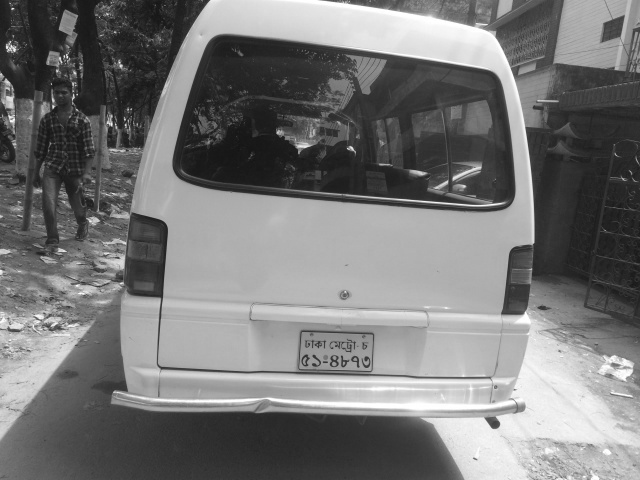
\includegraphics[width=0.9\linewidth]{./img/experiment/stage.2/angle}
    \caption{Original image}
\end{subfigure}
\begin{subfigure}{0.5\textwidth}
    \centering
    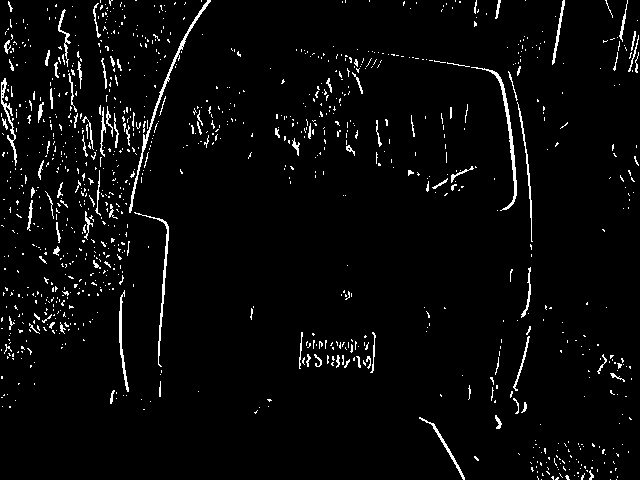
\includegraphics[width=0.9\linewidth]{./img/experiment/stage.3/angle}
    \caption{Edge image}
\end{subfigure}
\caption{Sobel image of a car with a slightly angled plate}
\label{fig:SobelResult1}
\end{figure}

\begin{figure}
\begin{subfigure}{0.5\textwidth}
    \centering
    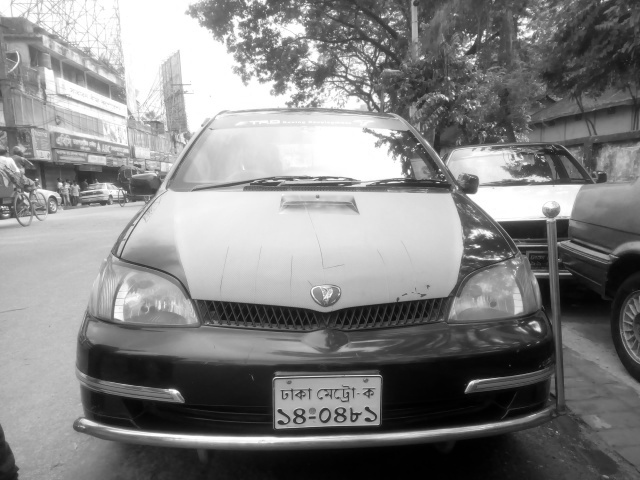
\includegraphics[width=0.9\linewidth]{./img/experiment/stage.2/good3}
    \caption{Original image}
\end{subfigure}
\begin{subfigure}{0.5\textwidth}
    \centering
    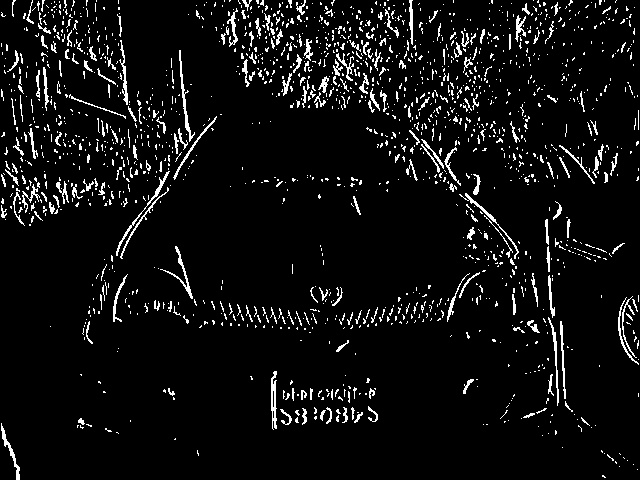
\includegraphics[width=0.9\linewidth]{./img/experiment/stage.3/good3}
    \caption{Edge image}
\end{subfigure}
\caption{Sobel image of a good plate image}
\label{fig:SobelResult2}
\end{figure}


\begin{figure}
\begin{subfigure}{0.5\textwidth}
    \centering
    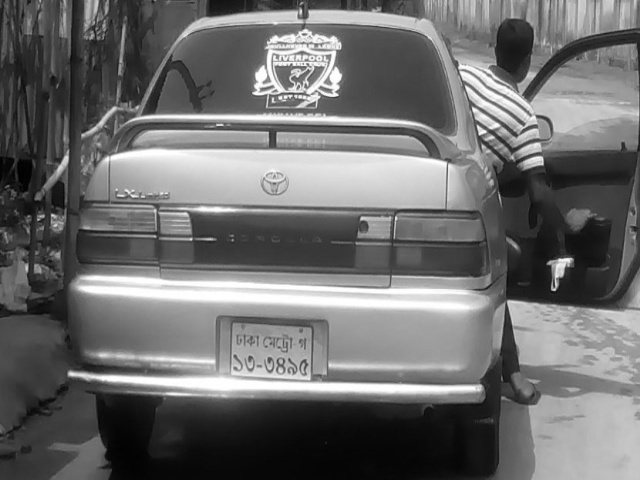
\includegraphics[width=0.9\linewidth]{./img/experiment/stage.2/light}
    \caption{Original image}
\end{subfigure}
\begin{subfigure}{0.5\textwidth}
    \centering
    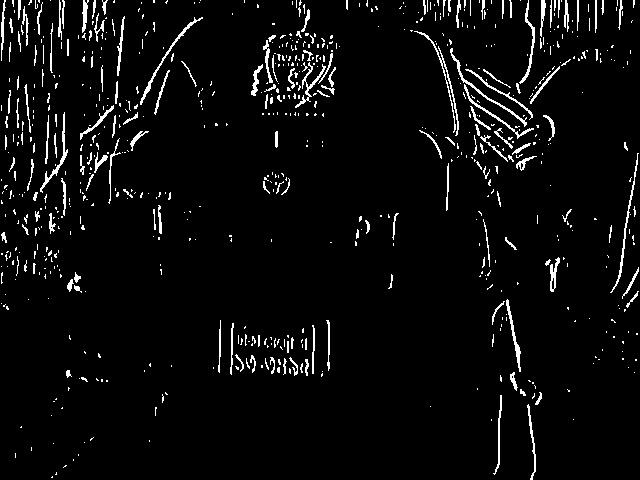
\includegraphics[width=0.9\linewidth]{./img/experiment/stage.3/light}
    \caption{Edge image}
\end{subfigure}
\caption{Sobel image of plate with light reflection}
\label{fig:SobelResult3}
\end{figure}

  \subsection{Gaussian Filter on Edge Image}
The Gaussian filter blurs the image. We observed that our filter blurs all of license plates on good samples, and only text portions on samples with larger plates. Figure \ref{fig:GaussianResult1}, \ref{fig:GaussianResult2} and \ref{fig:GaussianResult3} demonstrate result of this filter.

\begin{figure}
\begin{subfigure}{0.5\textwidth}
    \centering
    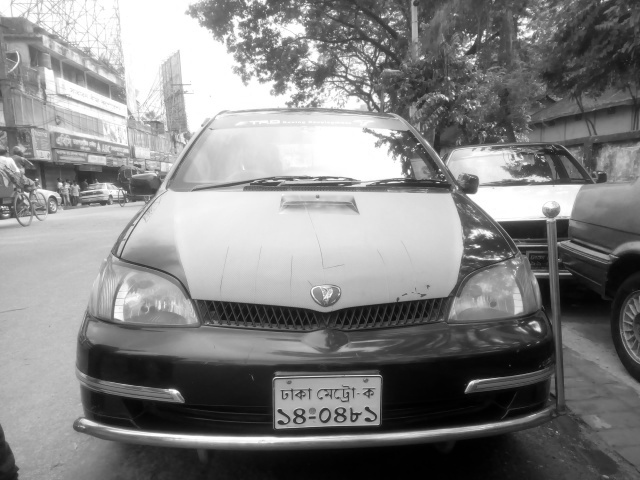
\includegraphics[width=0.9\linewidth]{./img/experiment/stage.2/good3}
    \caption{Original image}
\end{subfigure}
\begin{subfigure}{0.5\textwidth}
    \centering
    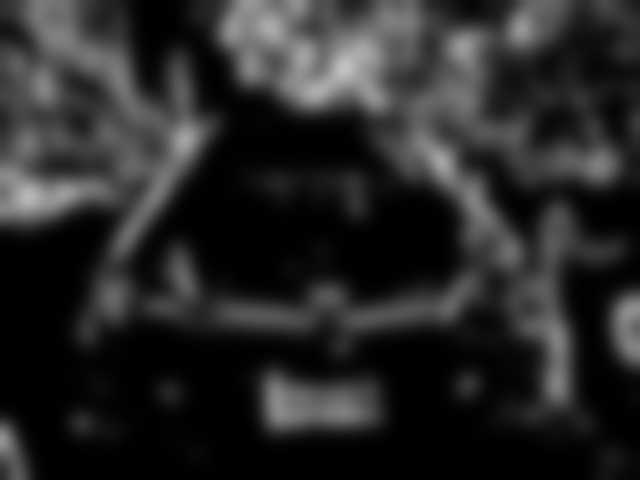
\includegraphics[width=0.9\linewidth]{./img/experiment/stage.4/good3}
    \caption{Blurry image}
\end{subfigure}
\caption{Gaussian filter on good plate}
\label{fig:GaussianResult1}
\end{figure}

\begin{figure}
\begin{subfigure}{0.5\textwidth}
    \centering
    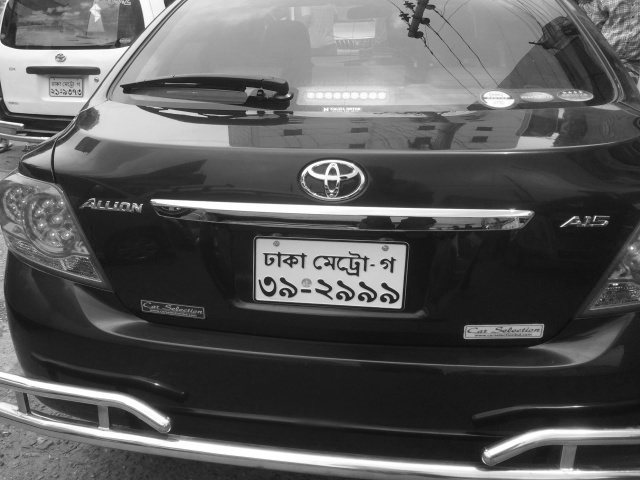
\includegraphics[width=0.9\linewidth]{./img/experiment/stage.2/angle3}
    \caption{Original image}
\end{subfigure}
\begin{subfigure}{0.5\textwidth}
    \centering
    
\includegraphics[width=0.9\linewidth]{./img/experiment/stage.4/angle3}
    \caption{Blurry image}
\end{subfigure}
\caption{Gaussian filter on big plate}
\label{fig:GaussianResult2}
\end{figure}

\begin{figure}
\begin{subfigure}{0.5\textwidth}
    \centering
    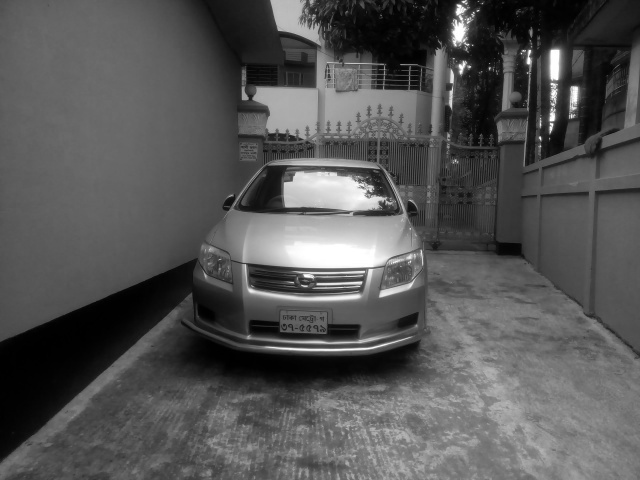
\includegraphics[width=0.9\linewidth]{./img/experiment/stage.2/small}
    \caption{Original image}
\end{subfigure}
\begin{subfigure}{0.5\textwidth}
    \centering
    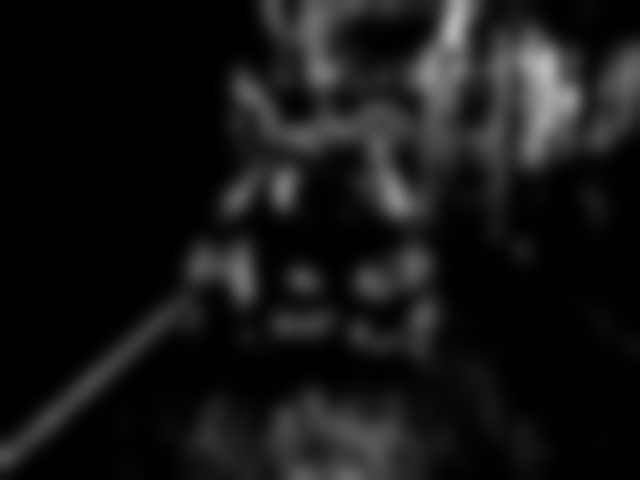
\includegraphics[width=0.9\linewidth]{./img/experiment/stage.4/small}
    \caption{Blurry image}
\end{subfigure}
\caption{Gaussian filter on small plate}
\label{fig:GaussianResult3}
\end{figure}

  \subsection{Enhanced Image vs original image}
If images are skewed or angled, this step does not work so well. Also, for small images and other images which has low blur around plate regions enhanced margin is low. Figure \ref{fig:EnhanceResult1}, \ref{fig:EnhanceResult2}, \ref{fig:EnhanceResult3} and \ref{fig:EnhanceResult4} demonstrate result of this step.

\begin{figure}
\begin{subfigure}{0.5\textwidth}
    \centering
    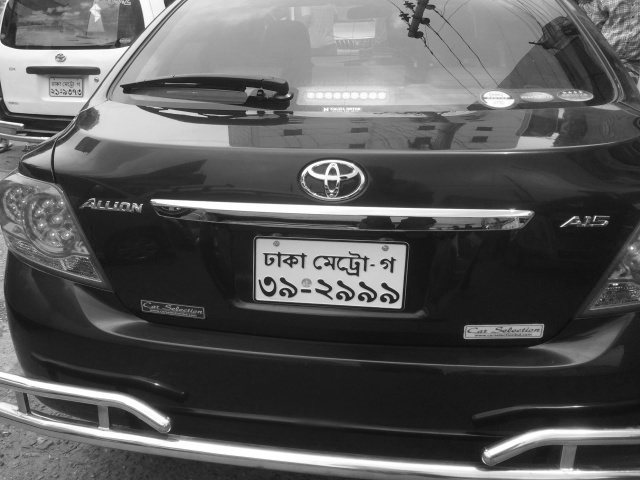
\includegraphics[width=0.9\linewidth]{./img/experiment/stage.2/angle3}
    \caption{Original image}
\end{subfigure}
\begin{subfigure}{0.5\textwidth}
    \centering
    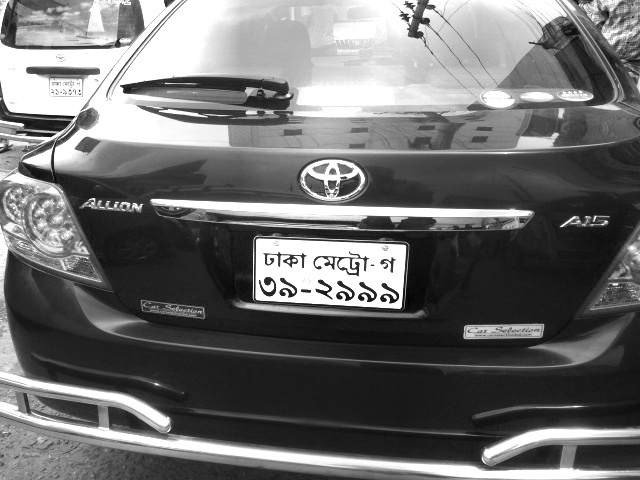
\includegraphics[width=0.9\linewidth]{./img/experiment/stage.5/angle3}
    \caption{Blurry image}
\end{subfigure}
\caption{Gaussian filter on good plate}
\label{fig:EnhanceResult1}
\end{figure}

\begin{figure}
\begin{subfigure}{0.5\textwidth}
    \centering
    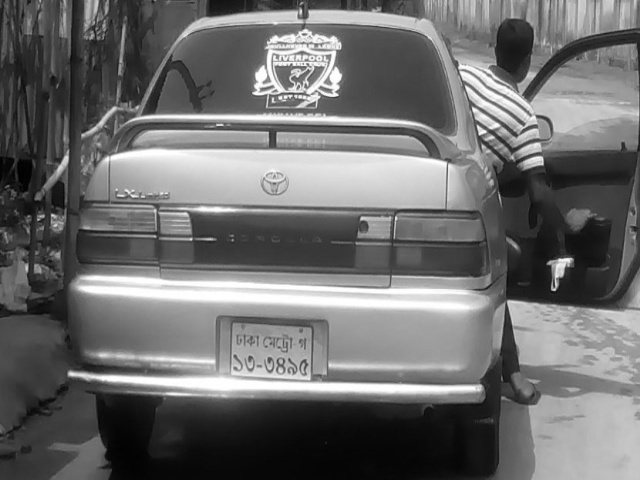
\includegraphics[width=0.9\linewidth]{./img/experiment/stage.2/light}
    \caption{Original image}
\end{subfigure}
\begin{subfigure}{0.5\textwidth}
    \centering
    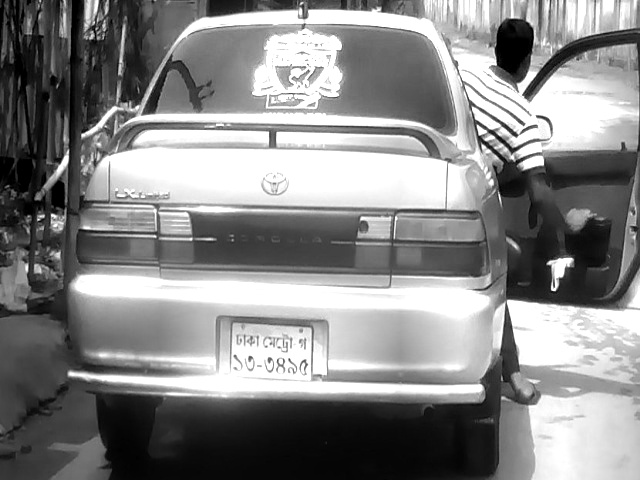
\includegraphics[width=0.9\linewidth]{./img/experiment/stage.5/light}
    \caption{Blurry image}
\end{subfigure}
\caption{Gaussian filter on plate with reflection}
\label{fig:EnhanceResult2}
\end{figure}

\begin{figure}
\begin{subfigure}{0.5\textwidth}
    \centering
    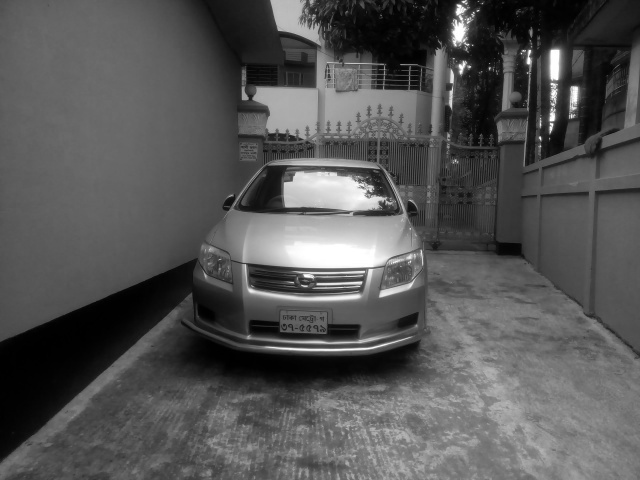
\includegraphics[width=0.9\linewidth]{./img/experiment/stage.2/small}
    \caption{Original image}
\end{subfigure}
\begin{subfigure}{0.5\textwidth}
    \centering
    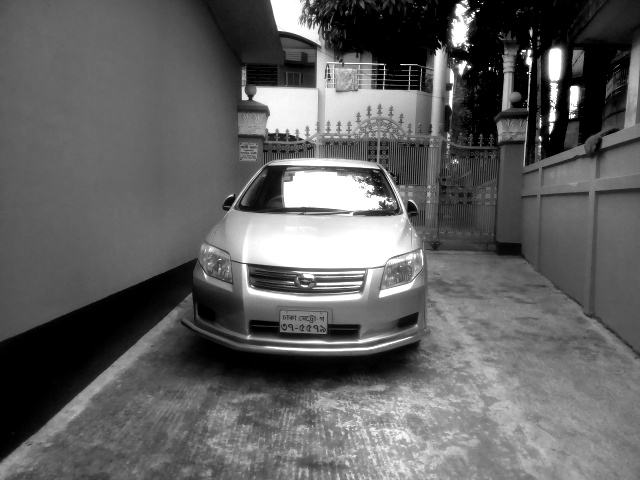
\includegraphics[width=0.9\linewidth]{./img/experiment/stage.5/small}
    \caption{Blurry image}
\end{subfigure}
\caption{Gaussian filter on small plate}
\label{fig:EnhanceResult3}
\end{figure}


\begin{figure}
\begin{subfigure}{0.5\textwidth}
    \centering
    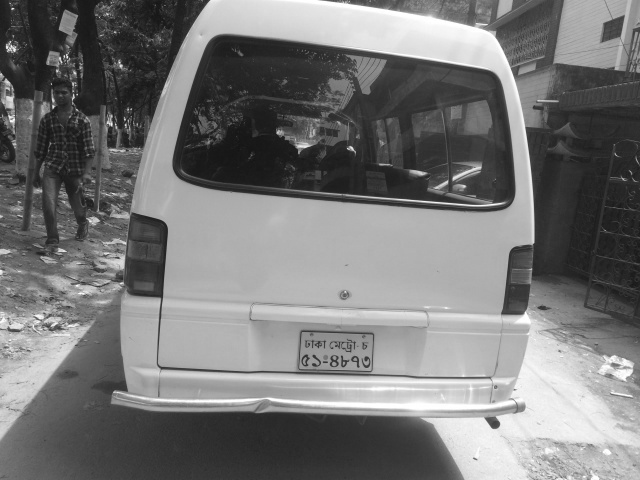
\includegraphics[width=0.9\linewidth]{./img/experiment/stage.2/angle}
    \caption{Original image}
\end{subfigure}
\begin{subfigure}{0.5\textwidth}
    \centering
    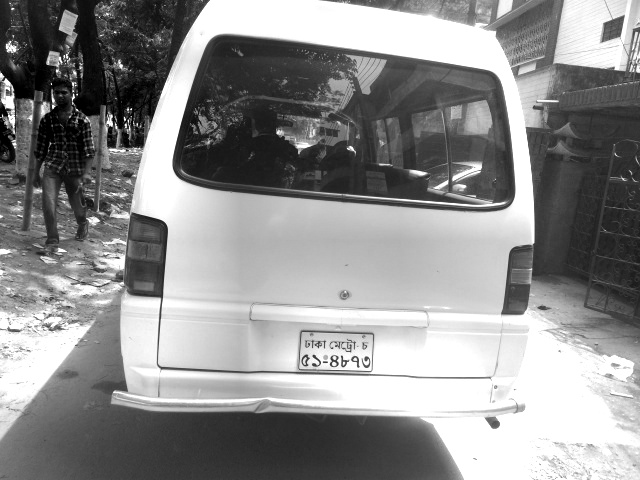
\includegraphics[width=0.9\linewidth]{./img/experiment/stage.5/angle}
    \caption{Blurry image}
\end{subfigure}
\caption{Gaussian filter on plate that is angled slightly}
\label{fig:EnhanceResult4}
\end{figure}

  \subsection{Matched filter on enhanced image}
Figure \ref{fig:MatchedResult1}, {fig:MatchedResult2}, {fig:MatchedResult3} show the result of this step.

\begin{figure}
\begin{subfigure}{0.5\textwidth}
    \centering
    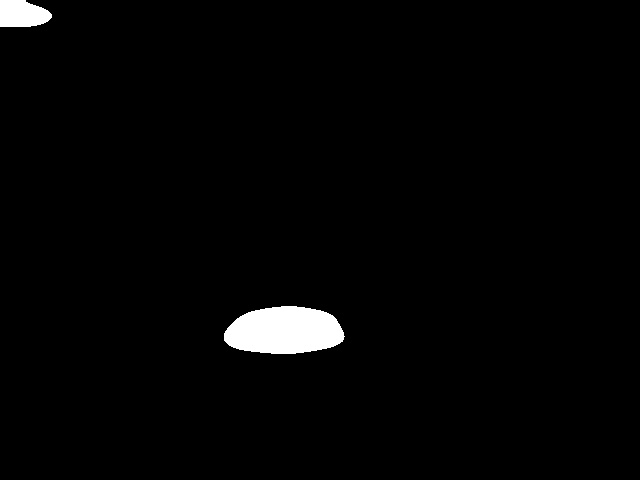
\includegraphics[width=0.9\linewidth]{./img/experiment/stage.6/good}
    \caption{Final result}
\end{subfigure}
\begin{subfigure}{0.5\textwidth}
    \centering
    \includegraphics[width=0.9\linewidth]{./img/experiment/stage.6/3-good}
    \caption{A see-through view with original image}
\end{subfigure}
\caption{After applying matched filter on a good image}
\label{fig:MatchedResult1}
\end{figure}

\begin{figure}
\begin{subfigure}{0.5\textwidth}
    \centering
    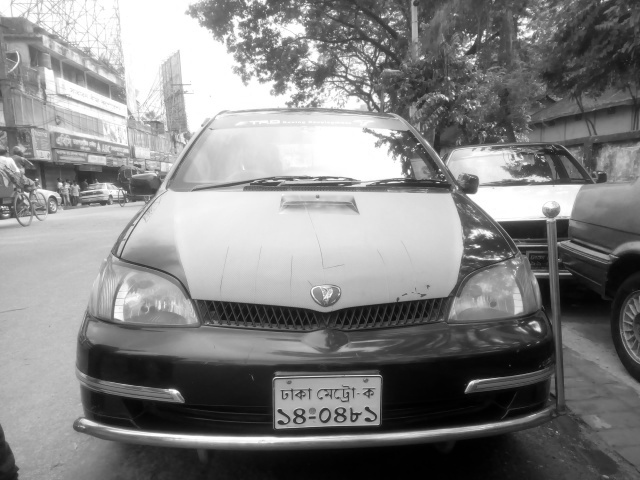
\includegraphics[width=0.9\linewidth]{./img/experiment/stage.2/good3}
    \caption{Original image}
\end{subfigure}
\begin{subfigure}{0.5\textwidth}
    \centering
    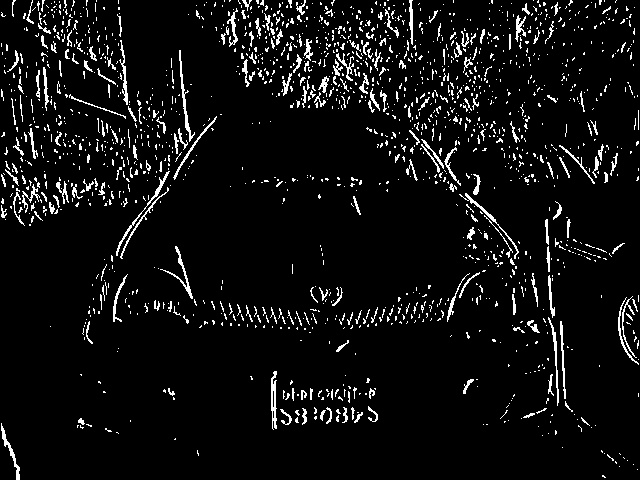
\includegraphics[width=0.9\linewidth]{./img/experiment/stage.3/good3}
    \caption{Edge image}
\end{subfigure}
\caption{Sobel image of a good plate image}
\label{fig:MatchedResult2}
\end{figure}


\begin{figure}
\begin{subfigure}{0.5\textwidth}
    \centering
    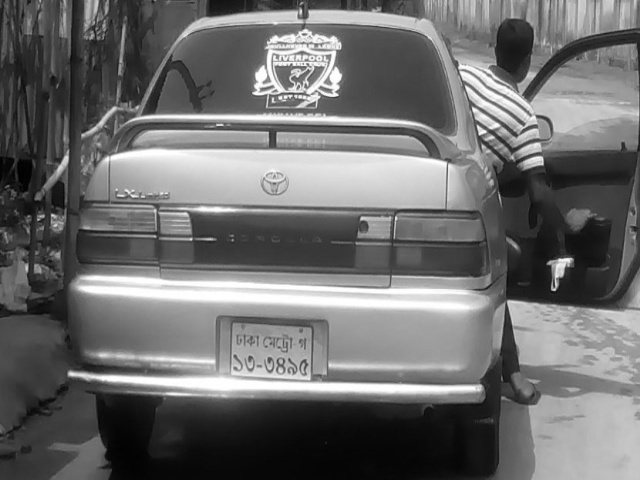
\includegraphics[width=0.9\linewidth]{./img/experiment/stage.2/light}
    \caption{Original image}
\end{subfigure}
\begin{subfigure}{0.5\textwidth}
    \centering
    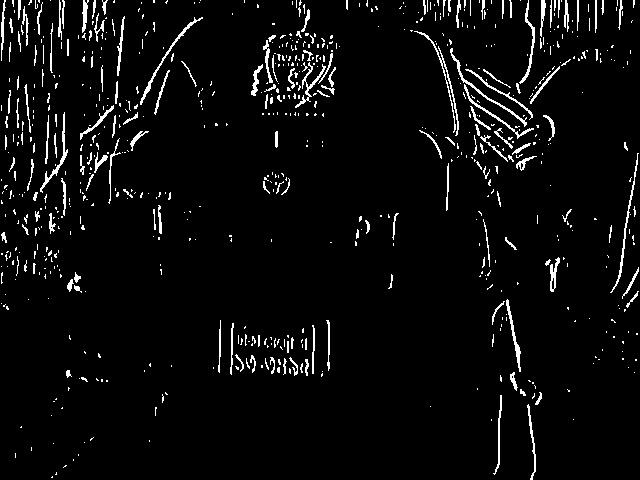
\includegraphics[width=0.9\linewidth]{./img/experiment/stage.3/light}
    \caption{Edge image}
\end{subfigure}
\caption{Sobel image of plate with light reflection}
\label{fig:MatchedResult3}
\end{figure}

  \subsection{Estimated plate regions}
Plate estimation is depended on the image found after applying matched filter. Bad plate images does not get enhanced well. Consequently it fails to have a good match on license plate regions and fails to locate exact positions of the plates. Good and bad results of this step is shown in Figure \ref{fig:Estimate1}, and \ref{fig:Estimate2}.

\begin{figure}
\begin{subfigure}{0.5\textwidth}
    \centering
    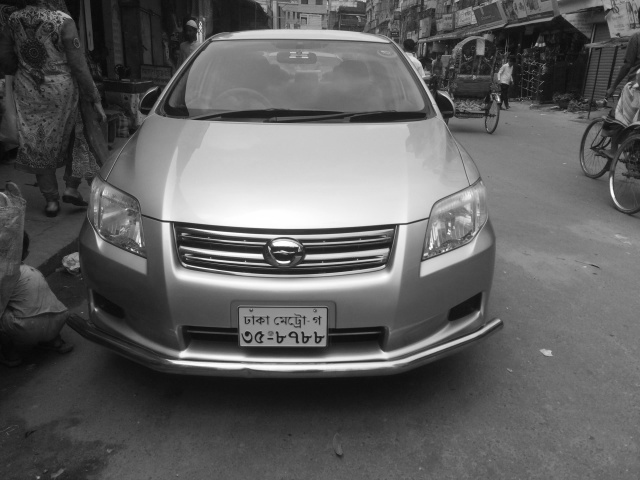
\includegraphics[width=0.9\linewidth]{./img/experiment/stage.2/good}
    \caption{Original image}
\end{subfigure}
\begin{subfigure}{0.5\textwidth}
    \centering
    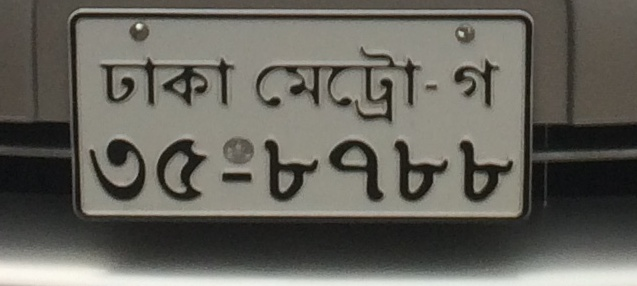
\includegraphics[width=0.9\linewidth]{./img/experiment/stage.8/00-good}
    \caption{The only estimated plate region}
\end{subfigure}
\caption{A good example of plate estimation}
\label{fig:Estimate1}
\end{figure}


\begin{figure}
\begin{subfigure}{0.5\textwidth}
    \centering
    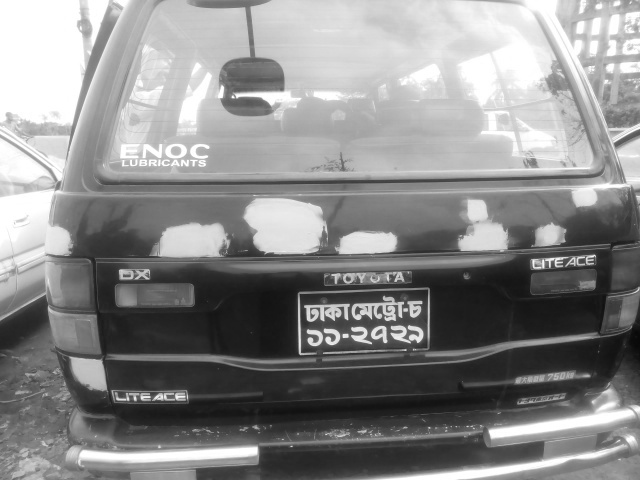
\includegraphics[width=0.9\linewidth]{./img/experiment/stage.2/private}
    \caption{Original image}
\end{subfigure}
\begin{subfigure}{0.24\textwidth}
    \centering
    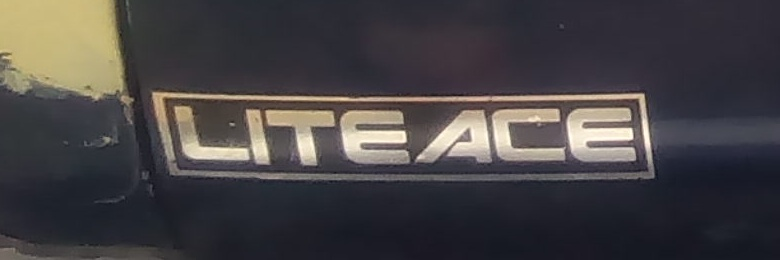
\includegraphics[width=0.9\linewidth]{./img/experiment/stage.8/00-private}
    \\ \vspace{0.3cm}
    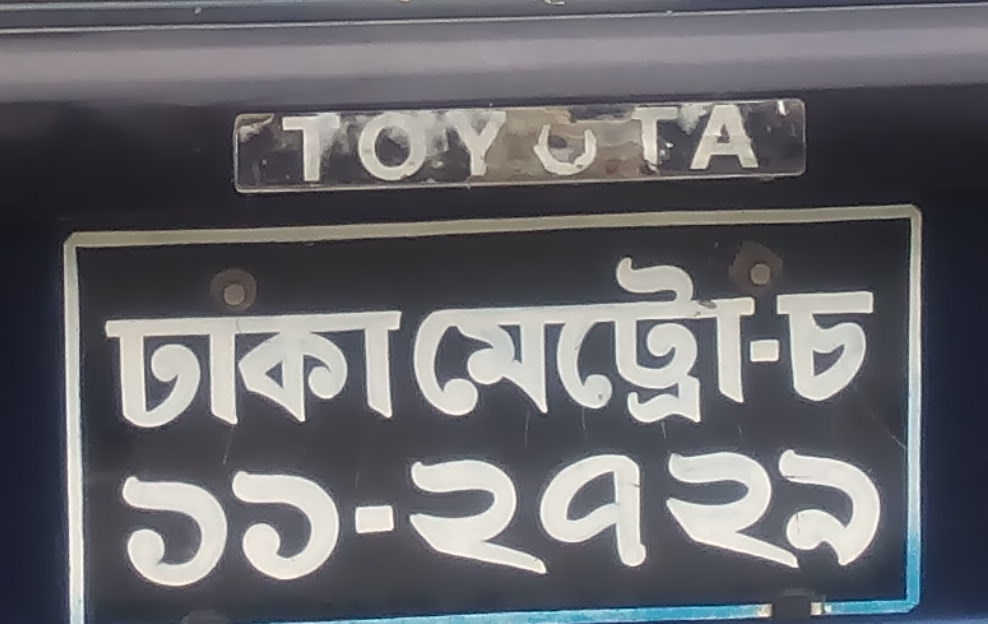
\includegraphics[width=0.9\linewidth]{./img/experiment/stage.8/02-private}
\end{subfigure}
\begin{subfigure}{0.24\textwidth}
    \centering
    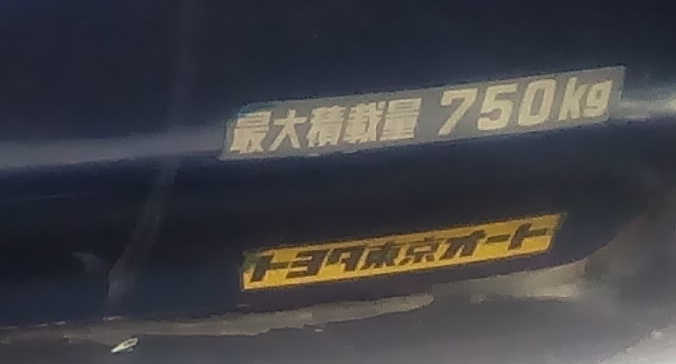
\includegraphics[width=0.9\linewidth]{./img/experiment/stage.8/01-private}
    \\ \vspace{0.3cm}
    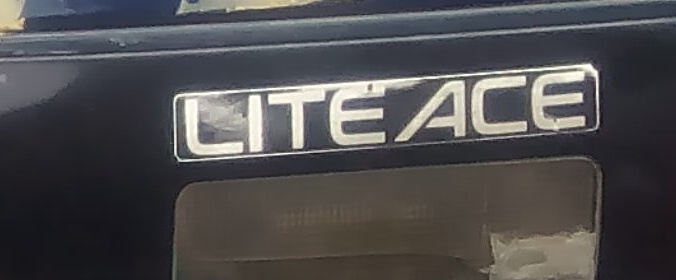
\includegraphics[width=0.9\linewidth]{./img/experiment/stage.8/03-private}
\end{subfigure}
\caption{Plate with lots of estimation}
\label{fig:Estimate2}
\end{figure}


\begin{figure}
\begin{subfigure}{0.5\textwidth}
    \centering
    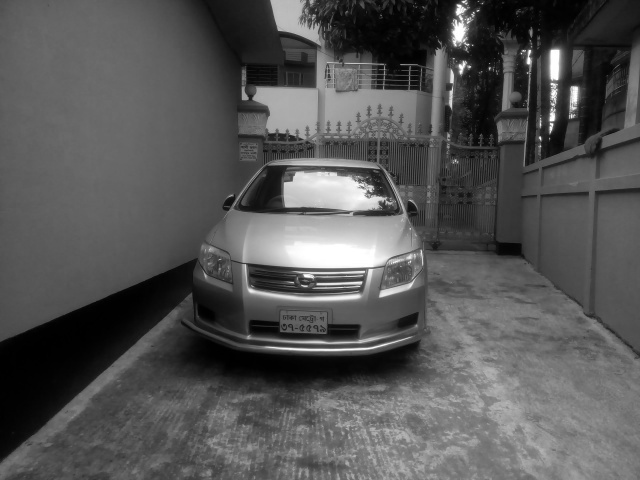
\includegraphics[width=0.9\linewidth]{./img/experiment/stage.2/small}
    \caption{Original image}
\end{subfigure}
\begin{subfigure}{0.24\textwidth}
    \centering
    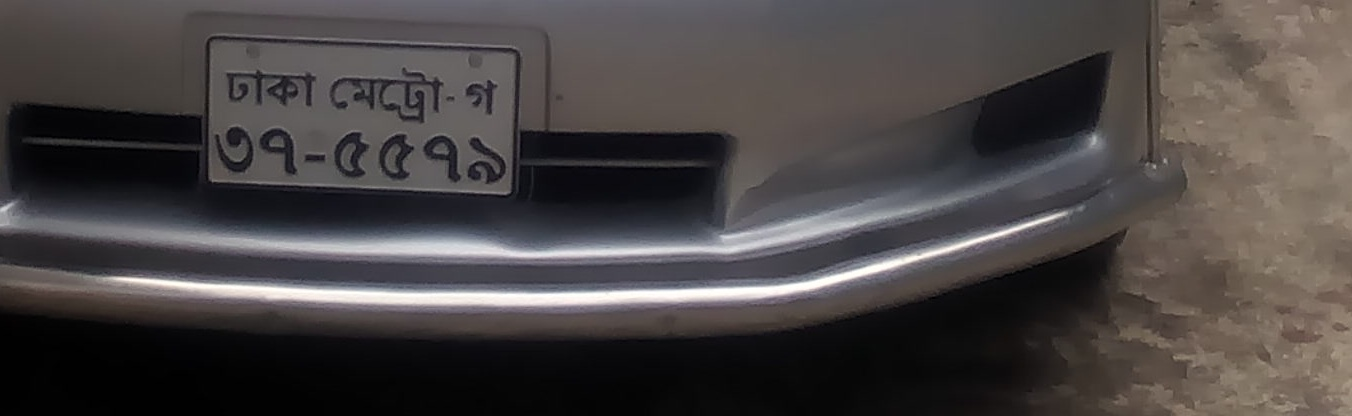
\includegraphics[width=0.9\linewidth]{./img/experiment/stage.8/00-small}
    \\ \vspace{0.3cm}
    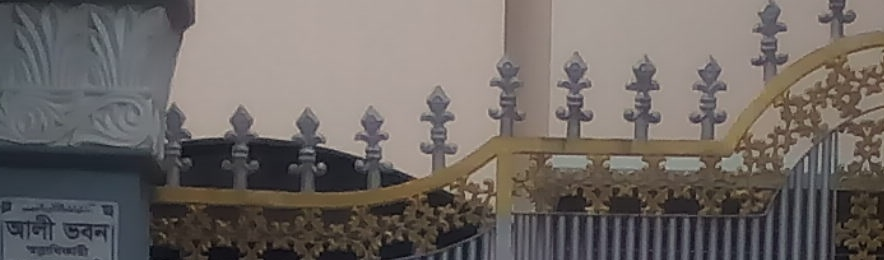
\includegraphics[width=0.9\linewidth]{./img/experiment/stage.8/02-small}
\end{subfigure}
\begin{subfigure}{0.24\textwidth}
    \centering
    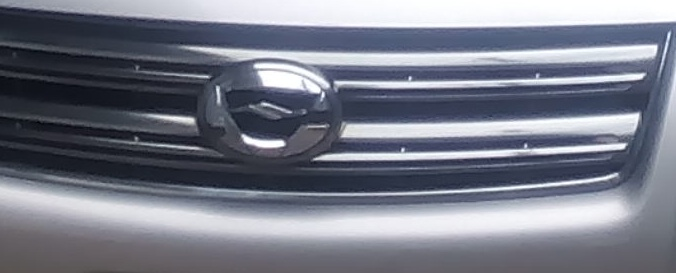
\includegraphics[width=0.9\linewidth]{./img/experiment/stage.8/01-small}
\end{subfigure}
\caption{Bad estimations}
\label{fig:Estimate2}
\end{figure}




\section{Plate Detection}
It takes every predicted plates and keeps only the text part of the plates. It also removes plates that can not be a possible plate.

  \subsection{Canny Edge Algorithm}
This algorithm is almost perfect for in detecting plate boundary. But if the plate is skewed or angled more tan 10 degrees it fails to draw a perfect boundary. In cases where the boundary is not inside the located region it also fails. Another backdrop is it draws double boundary for a plate for most of the cases. 

In Figure \ref{fig:CannyResult1}, \ref{fig:CannyResult2}, \ref{fig:CannyResult3}, and \ref{fig:CannyResult4} the results of the algorithm is shown.



\begin{figure}
\begin{subfigure}{0.33\textwidth}
    \centering
    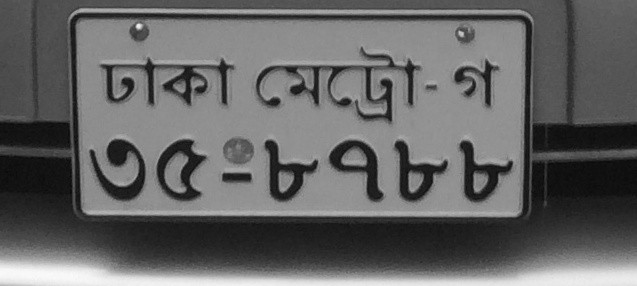
\includegraphics[width=0.9\linewidth]{./img/experiment/stage.9/00-good}
    \caption{Original}
\end{subfigure}
\begin{subfigure}{0.33\textwidth}
    \centering
    
\includegraphics[width=0.9\linewidth]{./img/experiment/stage.10/00-good}
    \caption{Threshold applied}
\end{subfigure}
\begin{subfigure}{0.33\textwidth}
    \centering
    
\includegraphics[width=0.9\linewidth]{./img/experiment/stage.11/00-good}
    \caption{Canny edges}
\end{subfigure}
\caption{Canny edges of a good plate}
\label{fig:CannyResult1}
\end{figure}


\begin{figure}
\begin{subfigure}{0.33\textwidth}
    \centering
    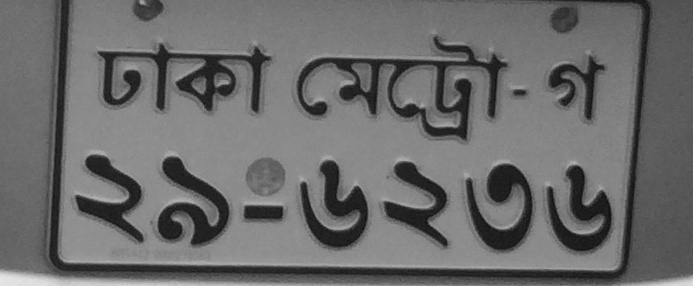
\includegraphics[width=0.9\linewidth]{./img/experiment/stage.9/00-angle2}
    \caption{Original}
\end{subfigure}
\begin{subfigure}{0.33\textwidth}
    \centering
    
\includegraphics[width=0.9\linewidth]{./img/experiment/stage.10/00-angle2}
    \caption{Threshold applied}
\end{subfigure}
\begin{subfigure}{0.33\textwidth}
    \centering
    
\includegraphics[width=0.9\linewidth]{./img/experiment/stage.11/00-angle2}
    \caption{Canny edges}
\end{subfigure}
\caption{Canny edges of an angled plate}
\label{fig:CannyResult2}
\end{figure}

\begin{figure}
\begin{subfigure}{0.33\textwidth}
    \centering
    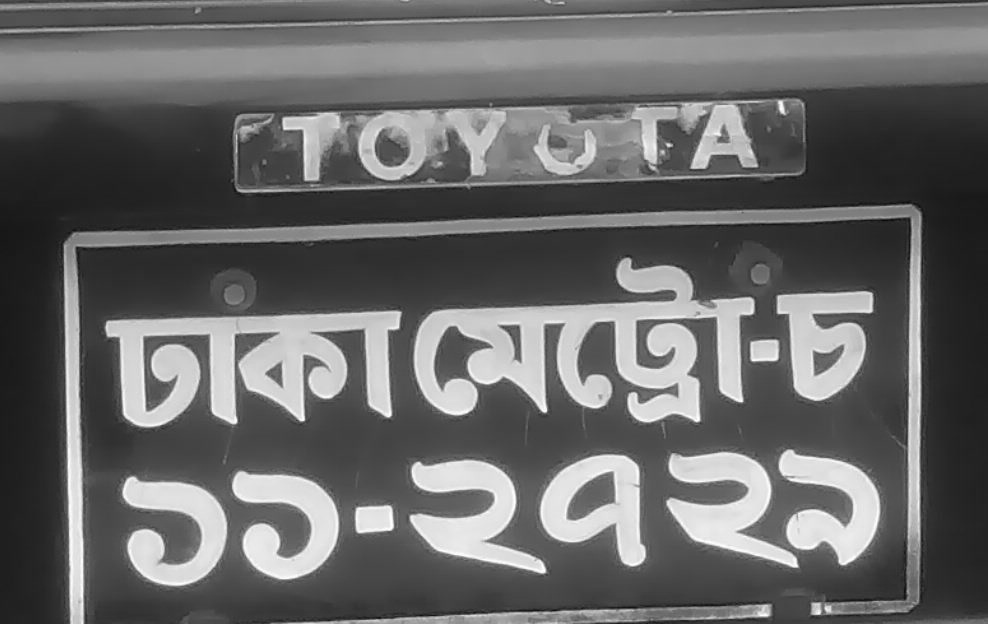
\includegraphics[width=0.9\linewidth]{./img/experiment/stage.9/02-private}
    \caption{Original}
\end{subfigure}
\begin{subfigure}{0.33\textwidth}
    \centering
    
\includegraphics[width=0.9\linewidth]{./img/experiment/stage.10/02-private}
    \caption{Threshold applied}
\end{subfigure}
\begin{subfigure}{0.33\textwidth}
    \centering
    
\includegraphics[width=0.9\linewidth]{./img/experiment/stage.11/02-private}
    \caption{Canny edges}
\end{subfigure}
\caption{Canny edges of a private plate}
\label{fig:CannyResult3}
\end{figure}


\begin{figure}
\begin{subfigure}{0.33\textwidth}
    \centering
    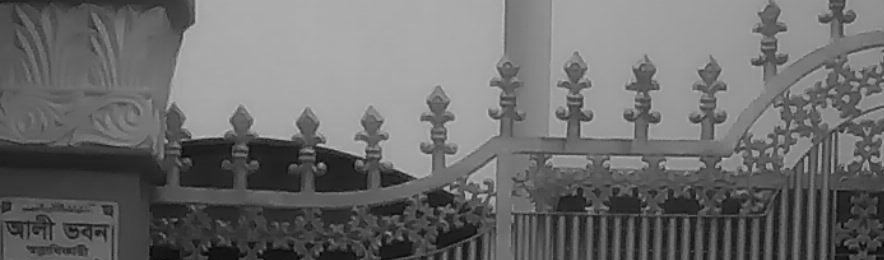
\includegraphics[width=0.9\linewidth]{./img/experiment/stage.9/02-small}
    \caption{Original}
\end{subfigure}
\begin{subfigure}{0.33\textwidth}
    \centering
    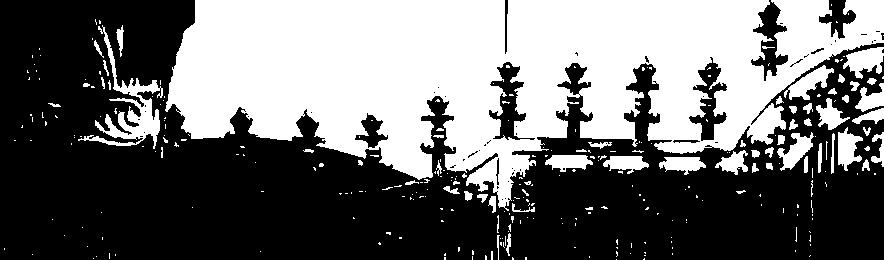
\includegraphics[width=0.9\linewidth]{./img/experiment/stage.10/02-small}
    \caption{Threshold applied}
\end{subfigure}
\begin{subfigure}{0.33\textwidth}
    \centering
    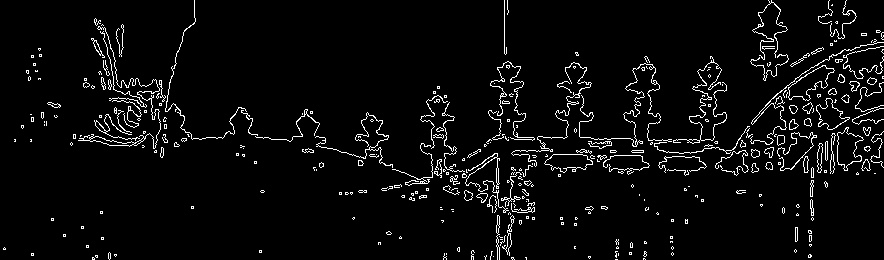
\includegraphics[width=0.9\linewidth]{./img/experiment/stage.11/02-small}
    \caption{Canny edges}
\end{subfigure}
\caption{Canny edges of a bad estimation}
\label{fig:CannyResult4}
\end{figure}


  \subsection{Contour Analysis}
The detection of contours vastly depended on the quality of edges detected by Canny edge detection algorithm. The contours can detect rotation, but we did not include the skew calculation. Rotation value fails in cases when the border of plate is not detected well or is out of the boundary of located plate region.

Figure \ref{fig:ContourResult1}, and \ref{fig:ContourResult2} shows two detected contour regions in each image. Contours are marked with a line of 2 pixels of black border upon 3 pixels of white border line.

\begin{figure}
\centering

\includegraphics[width=0.8\textwidth]{./img/experiment/stage.12/00-good}   
\caption{Two detected contours of a good sample}
\label{fig:ContourResult1}
\end{figure}

\begin{figure}
\centering
\includegraphics[width=0.8\textwidth]{./img/experiment/stage.12/00-private2}
\caption{Detected contours of a private plate}
\label{fig:ContourResult2}
\end{figure}


  \subsection{Extracted plates}
The extracted plate is also rotated according on contour data. If the contour fails to be detected properly, this also fails. Figure \ref{fig:ExtractedResult1}, \ref{fig:ExtractedResult2}, \ref{fig:ExtractedResult3}, and \ref{fig:ExtractedResult4} have some experimental results of the extracted plates.

\begin{figure}
\begin{subfigure}{0.5\textwidth}
    \centering
    \includegraphics[width=0.9\linewidth]{./img/experiment/stage.10/00-good}
    \caption{Original Plate}
\end{subfigure}
\begin{subfigure}{0.5\textwidth}
    \centering
    \includegraphics[width=0.9\linewidth]{./img/experiment/stage.13/00-00-good}
    \caption{Sole extracted image}
\end{subfigure}
\caption{Extracted parts of a good estimation}
\label{fig:ExtractedResult1}
\end{figure}

\begin{figure}
\begin{subfigure}{\textwidth}
    \centering
    \includegraphics[width=0.5\linewidth]{./img/experiment/stage.10/00-good3}
    \caption{Original Plate}
\end{subfigure}
\begin{subfigure}{0.5\textwidth}
    \centering
    \includegraphics[width=0.9\linewidth]{./img/experiment/stage.13/00-00-good3}
    \caption{First extracted image}    
\end{subfigure}
\begin{subfigure}{0.5\textwidth}
    \centering
    \includegraphics[width=0.9\linewidth]{./img/experiment/stage.13/01-00-good3}
    \caption{Second extracted image}
\end{subfigure}
\caption{Extracted parts of another good estimation}
\label{fig:ExtractedResult2}
\end{figure}


\begin{figure}
\begin{subfigure}{\textwidth}
    \centering
    \includegraphics[width=0.5\linewidth]{./img/experiment/stage.10/00-angle}
    \caption{Original Plate}
\end{subfigure}
\begin{subfigure}{0.5\textwidth}
    \centering
    \includegraphics[width=0.9\linewidth]{./img/experiment/stage.13/00-00-angle}
    \caption{First extracted image}
\end{subfigure}
\begin{subfigure}{0.5\textwidth}
    \centering
    \includegraphics[width=0.9\linewidth]{./img/experiment/stage.13/01-00-angle}
    \caption{Second extracted image}
\end{subfigure}
\caption{Extracted parts of angled plate}
\label{fig:ExtractedResult3}
\end{figure}


\begin{figure}
\begin{subfigure}{\textwidth}
    \centering
    \includegraphics[width=0.5\linewidth]{./img/experiment/stage.10/02-private}
    \caption{Original Plate}
\end{subfigure}
\begin{subfigure}{0.5\textwidth}
    \centering
    \includegraphics[width=0.9\linewidth]{./img/experiment/stage.13/00-02-private}
    \caption{First extracted image}
\end{subfigure}
\begin{subfigure}{0.5\textwidth}
    \centering
    \includegraphics[width=0.9\linewidth]{./img/experiment/stage.13/01-02-private}
    \caption{Second extracted image}
\end{subfigure}
\caption{Extracted parts of a private plate}
\label{fig:ExtractedResult4}
\end{figure}




  \subsection{Clean Plates}
After extracting plates the plates are converted into binary. This process has no failures. However the cleaning part has some critical cases. When the text is too close border, a portion of it gets erased. Also, sometimes if noise density and size large it is assumed to be a character and does not get erased. All such cases are shown in Figure \ref{fig:Cleaning1}, \ref{fig:Cleaning2}, and \ref{fig:Cleaning3}.


\begin{figure}
\begin{subfigure}{0.33\textwidth}
    \centering
    \includegraphics[width=0.9\linewidth]{./img/experiment/stage.14/01-00-good}
    \caption{Binary image}
\end{subfigure}
\begin{subfigure}{0.33\textwidth}
    \centering
    \includegraphics[width=0.9\linewidth]{./img/experiment/stage.15/01-00-good}
    \caption{Removed Borders}
\end{subfigure}
\begin{subfigure}{0.33\textwidth}
    \centering
    \includegraphics[width=0.9\linewidth]{./img/experiment/stage.16/01-00-good}
    \caption{Final image}
\end{subfigure}
\caption{Result of good cleaning}
\label{fig:Cleaning1}
\end{figure}

\begin{figure}
\begin{subfigure}{0.33\textwidth}
    \centering
    \includegraphics[width=0.9\linewidth]{./img/experiment/stage.14/01-00-private2}
    \caption{Binary image}
\end{subfigure}
\begin{subfigure}{0.33\textwidth}
    \centering
    \includegraphics[width=0.9\linewidth]{./img/experiment/stage.15/01-00-private2}
    \caption{Removed Borders}
\end{subfigure}
\begin{subfigure}{0.33\textwidth}
    \centering
    \includegraphics[width=0.9\linewidth]{./img/experiment/stage.16/01-00-private2}
    \caption{Final image}
\end{subfigure}
\caption{Result of bad cleaning}
\label{fig:Cleaning2}
\end{figure}


\begin{figure}
\begin{subfigure}{0.33\textwidth}
    \centering
    \includegraphics[width=0.9\linewidth]{./img/experiment/stage.14/00-00-good3}
    \caption{Binary image}
\end{subfigure}
\begin{subfigure}{0.33\textwidth}
    \centering
    \includegraphics[width=0.9\linewidth]{./img/experiment/stage.15/00-00-good3}
    \caption{Removed Borders}
\end{subfigure}
\begin{subfigure}{0.33\textwidth}
    \centering
    \includegraphics[width=0.9\linewidth]{./img/experiment/stage.16/00-00-good3}
    \caption{Final image}
\end{subfigure}
\caption{Cleaning an skewed plate}
\label{fig:Cleaning3}
\end{figure}


  

\section{Segmentation}  
Horizontal and vertical project are not perfect for skewed and angled plates. It also fails in case there are induced noise on license plate. Also if two characters overlaps each other in vertical direction (which is very common in bangla text) it also fails. Figure \ref{fig:SegmentResult1} shows an example of successful segmentation. When two characters overlaps the segmentation fails. An example is shown in Figure \ref{fig:OverlappingChar}. Also, non-standard plate like Figure \ref{fig:NonStandardPlates}.


\begin{figure}
\begin{subfigure}{\textwidth}
    \centering
    \includegraphics[width=0.5\linewidth]{./img/experiment/stage.16/01-00-good}
    \caption{Original Plate}
\end{subfigure}
\begin{subfigure}{0.15\textwidth}
    \centering
    \includegraphics[width=0.9\linewidth]{./img/experiment/stage.17/00-01-00-good}
\end{subfigure}
\begin{subfigure}{0.15\textwidth}
    \centering
    \includegraphics[width=0.9\linewidth]{./img/experiment/stage.17/01-01-00-good}
\end{subfigure}
\begin{subfigure}{0.09\textwidth}
    \centering
    \includegraphics[width=0.9\linewidth]{./img/experiment/stage.17/02-01-00-good}
\end{subfigure}
\begin{subfigure}{0.09\textwidth}
    \centering
    \includegraphics[width=0.9\linewidth]{./img/experiment/stage.17/03-01-00-good}
\end{subfigure}
\begin{subfigure}{0.09\textwidth}
    \centering
    \includegraphics[width=0.9\linewidth]{./img/experiment/stage.17/04-01-00-good}
\end{subfigure}
\begin{subfigure}{0.09\textwidth}
    \centering
    \includegraphics[width=0.9\linewidth]{./img/experiment/stage.17/05-01-00-good}
\end{subfigure}
\begin{subfigure}{0.09\textwidth}
    \centering
    \includegraphics[width=0.9\linewidth]{./img/experiment/stage.17/06-01-00-good}
\end{subfigure}
\begin{subfigure}{0.09\textwidth}
    \centering
    \includegraphics[width=0.9\linewidth]{./img/experiment/stage.17/07-01-00-good}
\end{subfigure}
\begin{subfigure}{0.09\textwidth}
    \centering
    \includegraphics[width=0.9\linewidth]{./img/experiment/stage.17/08-01-00-good}
\end{subfigure}
\caption{Segmented characters from a plate}
\label{fig:SegmentResult1}
\end{figure}


\begin{figure}
\begin{subfigure}{0.33\textwidth}
    \centering
    \includegraphics[width=0.9\linewidth]{./img/experiment/stage.17/06-00-00-badfont}
    \caption{Bad font}
\end{subfigure}
\begin{subfigure}{0.33\textwidth}
    \centering
    \includegraphics[width=0.9\linewidth]{./img/experiment/stage.17/07-01-00-private2}
    \caption{Skewed}
\end{subfigure}
\begin{subfigure}{0.33\textwidth}
    \centering
    \includegraphics[width=0.9\linewidth]{./img/experiment/stage.17/06-01-02-private}
    \caption{Non-standard font}
\end{subfigure}
\caption{Segmentation failed due to overlapping characters}
\label{fig:OverlappingChar}
\end{figure}


\begin{figure}
\centering
\includegraphics[width=0.5\linewidth]{./img/experiment/stage.16/01-00-nostd}    
\caption{Segmentation fails for non-standard plates}
\label{fig:NonStandardPlates}
\end{figure}




\section{Character Recognition}
The character recognition is done by neural network which is highly depended on training dataset. Unfortunately, we did not have enough dataset to train our neural network well to be able to produce any significant results. Our future goal includes this part of collecting dataset, and training and testing the neural network we implemented.


\section{Efficiency Measurements}


\end{document}